\documentclass[12pt]{article}
\usepackage{tikz}
\usetikzlibrary{bayesnet}
\usepackage{amsmath}
\begin{document}

\section*{Divisive Normalization Notes}

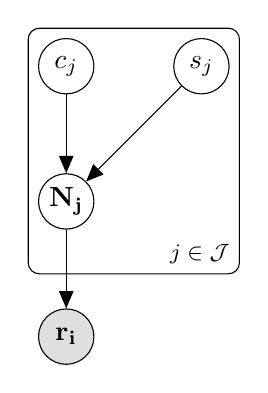
\begin{tikzpicture}

  % Define nodes
  \node[obs]                               (r) {$\mathbf{r_i}$};
  \node[latent, above=of r]        (N) {$\mathbf{N_j}$};
  \node[latent, above=of N] (c) {$c_j$};
  \node[latent, right=of c]  (s) {$s_j$};
  % Connect the nodes
  \edge {c,s} {N} ;
  \edge {N} {r} ; 
  \plate {} {(c) (s) (N)} {$j \in \mathcal{J}$};

\end{tikzpicture}
\\
$s_1 \sim \text{Unif}(-60, 60)$\\
$s_2 \sim \text{Unif}(s_1, 60)$\\
$N_{1, 2}$ is the response of neurons to grating 1, 2\\ 
(Poisson neurons with Gaussian tuning curves)\\
$r$ is response of neurons ($\sum N$)\\
\\

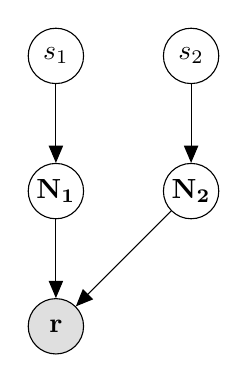
\begin{tikzpicture}

  % Define nodes
  \node[latent]  (s1) {$s_1$};
  \node[latent, below=of s1]        (N1) {$\mathbf{N_1}$};
  \node[latent, right=of s1]  (s2) {$s_2$};
  \node[latent, below=of s2]        (N2) {$\mathbf{N_2}$};
  \node[obs, below=of N1]                               (r) {$\mathbf{r}$};
  % Connect the nodes
  \edge {s1} {N1} ;
  \edge {s2} {N2} ;
  \edge {N1} {r} ; 
  \edge {N2} {r} ; 

\end{tikzpicture}
\\
\\

$\hat{\mathbf{s}} = \arg\max_\mathbf{s} p(\mathbf{r|s}) p(\mathbf{s})$
\\
\\
$\mathbf{r_\text{hid}} = \phi (\mathbf{W_{\text{hid}}r + b})$
\\
\\
$\mathbf{r} = \text{Poisson} (g_1\mathbf{f} (s_1) + g_2\mathbf{f} (s_2))$
\\
\\
$\hat{s_1}$
\\
\\
$\hat{s_2}$
\\
\\
$f_i(s)$ is tuning curve of neuron i\\
Tuning curve assumptions:\\
Tuning curves cover the space so $\sum_i f_i(s_j)$ is independent of $s_j$\\
The tuning curves are von Mises: $f_i(s_j) = e^{\kappa(\cos(s_j - s_i^{\text{pref}}) - 1)}$\\
$N_{ij}$ is the response of neuron i to grating j\\
$P(N|c, s) = \prod_i \text{Poisson}(N_{j}; f_i(s_j)c_j)$\\
$P(c) = \text{Gamma}(c_j; \alpha, \beta)$\\
$P(s) = \text{Unif}(0, 2\pi)$\\
\begin{equation}
\begin{aligned}
P(\mathbf{c, s|r}) & = \sum_N P(\mathbf{N, c, s|r}) = \sum_N P(\mathbf{r|N}) P(\mathbf{N|c, s}) P(\mathbf{c}) P(\mathbf{s})\\
&\propto \prod_i (\delta(r_i - \sum_j N_{ij}) \prod_j\frac{(f_i(s_j)c_j)^{N_{ij}} e^{-f_i(s_j) c_j}}{N_{ij}!}) (\prod_j \frac{\beta^{\alpha}}{\Gamma(\alpha)} c_j^{\alpha - 1}e^{\beta c_j})\\
\end{aligned}
\end{equation}
For the variational inference, we need\\
\begin{equation}
\begin{aligned}
\log P(\mathbf{N, c, s| r}) &= \sum_i [\log(\delta(r_i - \sum_j N_{ij})) - \sum_j [- \log N_{ij}! + N_{ij} \log(f_i(s_j)c_j) - f_i(s_j) c_j]]\\
& \phantom{{}=1} + \sum_j[(\alpha - 1) \log c_j - \beta c_j - \log (\beta^{- \alpha} \Gamma (\alpha))]\\
\end{aligned}
\end{equation}
Then we approximate this using a factorized distribution:\\
\begin{equation}
Q(\mathbf{N, c, s|r}) = Q(\mathbf{N|r}) Q(\mathbf{c|r}) Q(\mathbf{s|r})
\end{equation}
Then
\begin{equation}
\begin{aligned}
\log Q(\mathbf{N|r}) &= \langle \log P(\mathbf{N, c, s|r}) \rangle_{Q(\mathbf{c|r})Q(\mathbf{s|r})}\\
&= \sum_i [\log(\delta(r_i - \sum_j N_{ij})) - \sum_j [N_{ij} \langle \log(f_i (s_j)) c_j \rangle_{Q(\mathbf{c|r})Q(\mathbf{s|r})} - \log N_{ij}!]]\\
\end{aligned}
\end{equation}
\begin{equation}
\begin{aligned}
\log Q(\mathbf{c|r}) &= \langle \log P(\mathbf{N, c, s|r}) \rangle_{Q(\mathbf{N|r})Q(\mathbf{s|r})}\\
&= \sum_{ij} [\langle N_{ij} \rangle_{Q(\mathbf{N|r})} \log c_j - \langle f_i (s_j)\rangle_{Q(\mathbf{s|r}}c_j]\\
& \phantom{{}=1}+ \sum_j [(\alpha - 1) \log c_j - \beta c_j - \log (\beta^{- \alpha} \Gamma (\alpha))]\\
&= \sum_{ij} [(\alpha + \langle N_{ij} \rangle_{Q(\mathbf{c|r})} - 1) \log c_j - (\beta + \langle f_i (s_j)\rangle_{Q(\mathbf{s|r})}) c_j]\\
& \phantom{{}=1}- \sum_j \log (\beta^{- \alpha} \Gamma (\alpha))\\
\end{aligned}
\end{equation}
\begin{equation}
\begin{aligned}
\log Q(\mathbf{s|r}) &= \langle \log P(\mathbf{N, c, s|r}) \rangle_{Q(\mathbf{N|r})Q(\mathbf{c|r})}\\
&= \sum_{ij} [\langle N_{ij} \rangle_{Q(\mathbf{N|r})} \log(f_i(s_j)) - f_i(s_j) \langle c_j \rangle_{Q(\mathbf{c|r})}] = \sum_{ij} [\langle N_{ij} \rangle_{Q(\mathbf{N|r})} \log(f_i(s_j))]\\
\end{aligned}
\end{equation}
Last equality is because of space covering assumption\\
\\
So $Q(\mathbf{N|r})$ is a multinomial, $Q(\mathbf{c|r})$ is a Gamma and $Q(\mathbf{s|r})$ is von Mises\\
\begin{equation}
Q(\mathbf{N|r}) = \prod_i \delta(r_i - \sum_j N_{ij}) r_i! \prod_j \frac{\langle (f_i (s_j) c_j) \rangle_{Q(\mathbf{c|r})Q(\mathbf{s|r})}^{N_{ij}}}{N_{ij}!}
\end{equation}
\begin{equation}
Q(\mathbf{c|r}) = \prod_j \text{Gamma} (c_j|\alpha + \langle N_{ij} \rangle_{Q(\mathbf{c|r})}, \beta + \langle f_i (s_j)\rangle_{Q(\mathbf{s|r}}))\\
\end{equation}
\begin{equation}
\begin{aligned}
Q(\mathbf{s|r}) &\propto \prod_j e^{\kappa(\sum_{ij} [\langle N_{ij} \rangle_{Q(\mathbf{N|r})} \cos(s_j - s_i^{\text{pref}})}\\
&= \prod_j e^{\kappa(\sum_{j} \langle N_{ij} \rangle_{Q(\mathbf{N|r})} (\cos s_j \cos s_i^{\text{pref}} + \sin s_j \sin s_i^{\text{pref}}))}\\
&= \prod_j e^{\kappa(\sum_j (\cos s_j \sum_i \langle N_{ij} \rangle_{Q(\mathbf{N|r})} \cos s_i^{\text{pref}} + \sin s_j \sum_i \langle N_{ij} \rangle_{Q(\mathbf{N|r})} \sin s_i^{\text{pref}})})\\
&= \prod_j e^{\kappa(\cos s_j \cos(\sum_i \langle N_{ij} \rangle_{Q(\mathbf{N|r})} s_i^{\text{pref}}) + \sin s_j \sin(\sum_i \langle N_{ij} \rangle_{Q(\mathbf{N|r})} s_i^{\text{pref}})}\\
&= \prod_j e^{\tilde{\kappa} \cos(s_j - \hat{s})}\\
\text{where } \hat{s} &= \sum_i \langle N_{ij} \rangle_{Q(\mathbf{N|r})} s_i^{\text{pref}}
\end{aligned}
\end{equation}
\\
Calculations with:
$P(r|c, s) = \prod_i \text{Poisson}(r_i; \phi(\sum_j f_i(s_j)c_j))$\\
\begin{equation}
\begin{aligned}
P(\mathbf{c, s|r}) & = P(\mathbf{r|c, s}) P(\mathbf{c}) P(\mathbf{s})\\
&\propto \prod_i\frac{(\phi(\sum_j(f_i(s_j)c_j)))^{r_i} e^{-\phi(\sum_j(f_i(s_j)c_j))}}{r_i!}) (\prod_j \frac{\beta^{\alpha}}{\Gamma(\alpha)} c_j^{\alpha - 1}e^{\beta c_j})\\
\end{aligned}
\end{equation}
\begin{equation}
\begin{aligned}
\log P(\mathbf{c, s| r}) &= \sum_i [- \log r_i! + r_i \log(\phi(\sum_j(f_i(s_j)c_j))) - (\phi(\sum_j(f_i(s_j)c_j)))]]\\
& \phantom{{}=1} + \sum_j[(\alpha - 1) \log c_j - \beta c_j - \log (\beta^{- \alpha} \Gamma (\alpha))]\\
\end{aligned}
\end{equation}
\begin{equation}
Q(\mathbf{c, s|r}) = Q(\mathbf{c|r}) Q(\mathbf{s|r})
\end{equation}
\begin{equation}
\begin{aligned}
\log Q(\mathbf{c|r}) &= \langle \log P(\mathbf{c, s|r}) \rangle_{Q(\mathbf{s|r})}\\
&= \sum_i [r_i \langle \log(\phi(\sum_j(f_i(s_j)c_j))) \rangle_{Q(\mathbf{s|r})} - \langle \phi(\sum_j(f_i(s_j)c_j))) \rangle_{Q(\mathbf{s|r})}]\\
& \phantom{{}=1}+ \sum_j [(\alpha - 1) \log c_j - \beta c_j - \log (\beta^{- \alpha} \Gamma (\alpha))]\\
\end{aligned}
\end{equation}
\begin{equation}
\begin{aligned}
\log Q(\mathbf{s|r}) &= \langle \log P(\mathbf{c, s|r}) \rangle_{Q(\mathbf{c|r})}\\
&= \sum_i [r_i \langle \log(\phi(\sum_j(f_i(s_j)c_j))) \rangle_{Q(\mathbf{c|r})} - \langle \log(\phi(\sum_j(f_i(s_j)c_j))) c_j \rangle_{Q(\mathbf{c|r})}]\\
\end{aligned}
\end{equation}
For later: consider with relative contrast (Dirichlet?)\\
\\
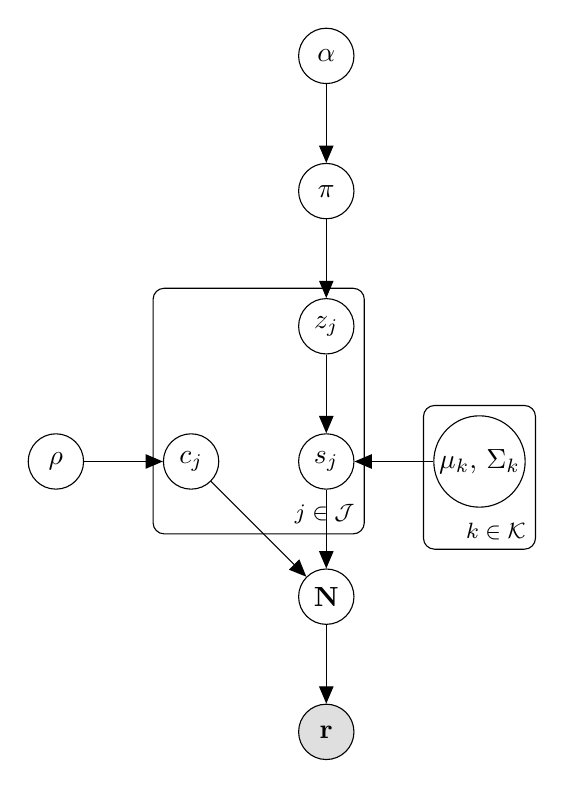
\begin{tikzpicture}

  % Define nodes
  \node[obs]                               (r) {$\mathbf{r}$};
  \node[latent, above=of r]        (N) {$\mathbf{N}$};
  \node[latent, above=of N] (s) {$s_j$};
  \node[latent, above=of s] (z) {$z_j$};
  \node[latent, above=of z] (pi) {$\pi$};
  \node[latent, above=of pi] (a) {$\alpha$};
  \node[latent, right=of s]  (th) {$\mu_k$, $\Sigma_k$};
  \node[latent, left=of s]  (c) {$c_j$};
  \node[latent, left=of c]  (rho) {$\rho$};
  % Connect the nodes
  \edge {c,s} {N};
  \edge {N} {r}; 
  \edge {rho} {c}; 
  \edge {pi} {z};
  \edge {a} {pi};
  \edge {z, th} {s}; 
  \plate {} {(c) (s) (z)} {$j \in \mathcal{J}$};
  \plate {} {(th)} {$k \in \mathcal{K}$};

\end{tikzpicture}
\\
$s_j|z_j \sim \mathcal{N}(\mu_{z_j}, \Sigma_{z_j})$\\
$N_{ij}|\{s_j\}  \sim \text{Poisson}(c_j f_i(s_j))$\\
$r_i|N_{ij} \sim \delta(r_i - z_j N_{ij})$\\
$\pi \sim \text{Dir} (\alpha)$\\
$c \sim \text{Dir} (\rho)$\\
\\
\begin{equation}
\begin{aligned}
\log Q(z) &= \langle \log P(z, s, c, \mu, \Sigma, N, r) \rangle_{Q(s)Q(N)Q(c)Q(\mu, \Sigma)}\\
&= \langle \log(\text{Mult}(z; \pi) \text{Dir}(\pi; \alpha) \prod_{j=1}^J \mathcal{N}(s_j; \mu_{z_j}, \Sigma_{z_j}) \text{Dir}(c, \rho)...\\
& \phantom{{}=1} \prod_{j=1}^J ((\delta(r_i - z_j N_{ij}) \text{Poisson}(c_j f_i(s_j)))...\\
& \phantom{{}=1} \prod_{k=1}^K \mathcal{N}(\mu_k; m_k, (\beta_0 \Sigma_k)) \text{Wi}(\Sigma_k^{-1}; \textbf{L}_0 ,\nu_0)) \rangle_{Q(s)Q(N)Q(c)Q(\mu, \Sigma)}\\
\end{aligned}
\end{equation}
\\
\begin{equation}
\begin{aligned}
\log Q(s) &= \langle \log \mathcal{N}(\mu_{z_j}, \Sigma_{z_j}) \rangle_{Q(z)Q(\mu, \Sigma)} + \sum_{i=1}^I \langle N_{ij} \log f_i(s_j) \rangle_{Q(N)}\\
&= - (\langle (s_j - \mu_j)^T \Sigma_{z_j}^{-1} (s_j - \mu_j) \rangle_{Q(z)Q(\mu, \Sigma)} + \sum_{i=1}^I \langle N_{ij} \rangle_{Q(N)} \log f_i(s_j))\\
&= - (\sum_{k=1}^K Q(z_j = k)\langle (s_j - \mu_j)^T \Sigma_{z_j}^{-1} (s_j - \mu_j) \rangle_{Q(\mu, \Sigma)} - \langle N_{ij} \rangle_{Q(N)} \frac{||(s_j - s_i^{\text{pref})}||^2}{L})\\
\end{aligned}
\end{equation}
\\
\begin{equation}
\begin{aligned}
\log Q(c) &= \langle \sum_j (\rho_j - 1) \log c_j \rangle + \sum_{ij} \langle N_{ij} \log c_j \rangle\\
&= \sum_j [\log c_j][\rho_j - 1 + \sum_i \langle N_{ij} \rangle
\end{aligned}
\end{equation}
\\
Redoing above with this graphical model:\\
\\
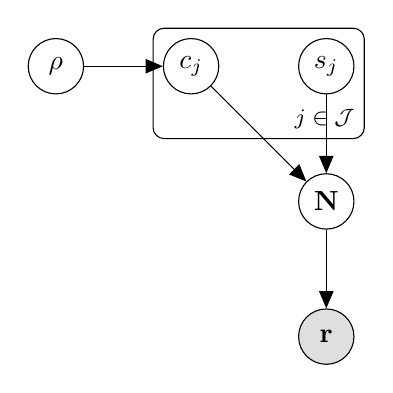
\begin{tikzpicture}
\node[obs]                               (r) {$\mathbf{r}$};
  \node[latent, above=of r]        (N) {$\mathbf{N}$};
  \node[latent, above=of N] (s) {$s_j$};
   \node[latent, left=of s]  (c) {$c_j$};
  \node[latent, left=of c]  (rho) {$\rho$};
   \edge {c,s} {N};
  \edge {N} {r}; 
  \edge {rho} {c}; 
  \plate {} {(c) (s)} {$j \in \mathcal{J}$};
 \end{tikzpicture}
 \\
$s_j$ is stimulus j\\
$c_j$ is contrast of grating j\\
$r_i$ is response of neuron i\\
$f_i(s)$ is tuning curve of neuron i\\
Tuning curve assumptions:\\
Tuning curves cover the space so $\sum_i f_i(s_j)$ is independent of $s_j$\\
The tuning curves are von Mises: $f_i(s_j) = e^{\kappa(\cos(s_j - s_i^{\text{pref}}) - 1)}$\\
$N_{ij}$ is the response of neuron i to grating j\\
$N_{ij}|\{s_j\}  \sim \text{Poisson}(c_j f_i(s_j))$\\
$r_i|N_{ij} \sim \delta(r_i - z_j N_{ij})$\\
$\pi \sim \text{Dir} (\alpha)$\\
$c \sim \text{Dir} (\rho)$\\
$s \sim \text{Unif} (0, \pi)$\\
\\
\begin{equation}
\begin{aligned}
P(\mathbf{c, s|r}) & = \sum_N P(\mathbf{N, c, s|r}) = \sum_N P(\mathbf{r|N}) P(\mathbf{N|c, s}) P(\mathbf{c}) P(\mathbf{s})\\
&\propto \prod_i (\delta(r_i - \sum_j N_{ij}) \prod_j\frac{(f_i(s_j)c_j)^{N_{ij}} e^{-f_i(s_j) c_j}}{N_{ij}!}) (\prod_j \frac{1}{\mathbf{\beta}(\rho)} c_j^{\rho - 1})\\
\end{aligned}
\end{equation}
\\
For the variational inference, we need\\
 \begin{equation}
\begin{aligned}
\log P(\mathbf{N, c, s| r}) &= \sum_i [\log(\delta(r_i - \sum_j N_{ij}))] - \sum_j [-\log N_{ij}! + N_{ij} \log(f_i(s_j)c_j)]\\
& \phantom{{}=1} + \sum_j [(\rho_j - 1)\log c_j]\\
\end{aligned}
\end{equation}
\\
Then we approximate this using a factorized distribution:\\
\begin{equation}
Q(\mathbf{N, c, s|r}) = Q(\mathbf{N|r}) Q(\mathbf{c|r}) Q(\mathbf{s|r})
\end{equation}
\\
\begin{equation}
\begin{aligned}
\log Q(\mathbf{N|r}) &= \langle \log P(\mathbf{N, c, s|r}) \rangle_{Q(\mathbf{c|r})Q(\mathbf{s|r})}\\
&= \sum_i [\log(\delta(r_i - \sum_j N_{ij})) - \sum_j [N_{ij} \langle \log(f_i (s_j)) c_j \rangle_{Q(\mathbf{c|r})Q(\mathbf{s|r})} - \log N_{ij}!]]\\
\end{aligned}
\end{equation}
\\
\begin{equation}
\begin{aligned}
\log Q(\mathbf{c|r}) &= \langle \log P(\mathbf{N, c, s|r}) \rangle_{Q(\mathbf{N|r})Q(\mathbf{s|r})}\\
&= \sum_j [\log c_j(\rho_j - 1 + \sum_i \langle N_{ij} \rangle_{Q(\mathbf{N|r}})]
\end{aligned}
\end{equation}
\\
\begin{equation}
\begin{aligned}
\log Q(\mathbf{s|r}) &= \langle \log P(\mathbf{N, c, s|r}) \rangle_{Q(\mathbf{N|r})Q(\mathbf{c|r})}\\
&= \sum_{ij} [\langle N_{ij} \rangle_{Q(\mathbf{N|r})} \log(f_i(s_j)) - f_i(s_j) \langle c_j \rangle_{Q(\mathbf{c|r})}] = \sum_{ij} [\langle N_{ij} \rangle_{Q(\mathbf{N|r})} \log(f_i(s_j))]\\
\end{aligned}
\end{equation}
\\
So $Q(\mathbf{N|r})$ is multinomial, $Q(\mathbf{c|r})$ is Dirichlet and $Q(\mathbf{s|r})$ is von Mises\\
\begin{equation}
Q(\mathbf{N|r}) = \prod_i \delta(r_i - \sum_j N_{ij}) r_i! \prod_j \frac{\langle (f_i (s_j) c_j) \rangle_{Q(\mathbf{c|r})Q(\mathbf{s|r})}^{N_{ij}}}{N_{ij}!}
\end{equation}
\begin{equation}
Q(\mathbf{c|r}) = \prod_j \text{Dir}(c_j; \rho_j - 1 + \sum_i \langle N_{ij} \rangle_{Q(\mathbf{N|r}})\\
\end{equation}
\\
\end{document}
